\documentclass{article}
\usepackage[utf8]{inputenc}
\usepackage[T1]{fontenc}
\usepackage{hyperref}
\usepackage{url}
\usepackage{booktabs}
\usepackage{amsfonts}
\usepackage{nicefrac}
\usepackage{microtype}

\usepackage{subcaption}
\usepackage{graphicx}
\usepackage{amsmath}
\usepackage{multirow}
\usepackage{color}
\usepackage{colortbl}
\usepackage{cleveref}
\usepackage{algorithm}
\usepackage{algorithmicx}
\usepackage{algpseudocode}

\DeclareMathOperator*{\argmin}{arg\,min}
\DeclareMathOperator*{\argmax}{arg\,max}

\graphicspath{{}}

\begin{filecontents}{references.bib}
@article{Buzsaki2002Theta,
  author = {Buzsáki, György},
  title = {Theta oscillations in the hippocampus},
  journal = {Neuron},
  year = {2002},
  volume = {33},
  number = {3},
  pages = {325--340},
}

@article{Canolty2006HighGamma,
  author = {Canolty, Ryan T. and Edwards, Erik and Dalal, Sarang S. and Soltani, Maryam and Nagarajan, Srikantan S. and Kirsch, Heidi E. and Berger, Mitchel S. and Barbaro, Nicholas M. and Knight, Robert T.},
  title = {High gamma power is phase-locked to theta oscillations in human neocortex},
  journal = {Science},
  year = {2006},
  volume = {313},
  number = {5793},
  pages = {1626--1628},
}

@article{Fell2010MedialTemporal,
  author = {Fell, Juergen and Ludowig, Eva and Staresina, Bernhard P. and Wagner, Tobias and Kranz, Thomas and Elger, Christian E. and Axmacher, Nikolai},
  title = {Medial temporal theta/alpha power enhancement preceding successful memory encoding: evidence based on intracranial EEG},
  journal = {NeuroImage},
  year = {2010},
  volume = {49},
  number = {3},
  pages = {2611--2617},
}

@article{Fries2005Gamma,
  author = {Fries, Pascal},
  title = {A mechanism for cognitive dynamics: neuronal communication through neuronal coherence},
  journal = {Trends in Cognitive Sciences},
  year = {2005},
  volume = {9},
  number = {10},
  pages = {474--480},
}

@article{Griffiths2019Directed,
  author = {Griffiths, Benjamin J. and Parish, George and Roux, Frédéric and Michelmann, Sebastian and van der Plas, Mirjam and Kolibius, Luca D. and Chelvarajah, Ramesh and Rollings, David T. and Sawlani, Vijay and Hamer, Hajo and Gollwitzer, Stephanie and Kreiselmeyer, Gernot and Staresina, Bernhard and Wimber, Maria and Hanslmayr, Simon},
  title = {Directional coupling between theta and gamma oscillations in the human hippocampus predicts memory performance},
  journal = {Nature Communications},
  year = {2019},
  volume = {10},
  pages = {5372},
}

@article{Hsieh2017Dynamic,
  author = {Hsieh, Liang-Tien and Ranganath, Charan},
  title = {Dynamic changes in hippocampal and prefrontal interactions during memory retrieval},
  journal = {Neurobiology of Learning and Memory},
  year = {2017},
  volume = {142},
  pages = {218--229}
}

@article{Johnson2020Replay,
  author = {Johnson, Adam and Redish, A. David},
  title = {Replay of memory sequences during hippocampal sharp-wave ripples},
  journal = {eLife},
  year = {2020},
  volume = {9},
  pages = {e53564}
}

@article{Manns2007Hippocampal,
  author = {Manns, Joseph R. and Eichenbaum, Howard},
  title = {Hippocampal representation of object-context associations},
  journal = {Learning \& Memory},
  year = {2007},
  volume = {14},
  number = {9},
  pages = {616--624}
}

@article{Norman2006Complementary,
  author = {Norman, Kenneth A. and O'Reilly, Randall C.},
  title = {Complementary learning systems in the brain: How the hippocampus and neocortex interact},
  journal = {Trends in Cognitive Sciences},
  year = {2006},
  volume = {10},
  number = {2},
  pages = {56--63}
}

@article{Ritchey2020Cortical,
  author = {Ritchey, Maureen and Yonelinas, Andrew P. and Ranganath, Charan},
  title = {Cortical representations of temporal context in episodic memory},
  journal = {NeuroImage},
  year = {2020},
  volume = {213},
  pages = {116735}
}

@article{Sederberg2007Gamma,
  author = {Sederberg, Per B. and Schulze-Bonhage, Andreas and Madsen, Joseph R. and Bromfield, Edward B. and McCarthy, David C. and Brandt, Armin and Tully, Michele S. and Kahana, Michael J.},
  title = {Gamma oscillations distinguish true from false memories},
  journal = {Psychological Science},
  year = {2017},
  volume = {18},
  number = {11},
  pages = {927--932}
}

@article{Siegle2011Enhancement,
  author = {Siegle, Joshua H. and Wilson, Matthew A.},
  title = {Enhancement of encoding and retrieval functions through theta phase-specific modulation of hippocampus},
  journal = {eLife},
  year = {2015},
  volume = {3},
  pages = {e04551}
}

@article{Singer1999Binding,
  author = {Singer, Wolf},
  title = {Neuronal synchrony: A versatile code for the definition of relations?},
  journal = {Neuron},
  year = {2019},
  volume = {24},
  number = {1},
  pages = {49--65}
}

@article{Sporns2016Modular,
  author = {Sporns, Olaf and Betzel, Richard F.},
  title = {Modular brain networks},
  journal = {Annual Review of Psychology},
  year = {2016},
  volume = {67},
  pages = {613--640}
}

@article{Staresina2015Reinstatement,
  author = {Staresina, Bernhard P. and Gray, John C. and Davachi, Lila},
  title = {Reinstatement of encoding context during retrieval},
  journal = {NeuroImage},
  year = {2015},
  volume = {116},
  pages = {10--18}
}









@article{ritchey2008cortical,
  author = {Ritchey, Maureen and Wing, Erik A. and LaBar, Kevin S. and Cabeza, Roberto},
  title = {Cortical reinstatement of episodic memory representations},
  journal = {Journal of Cognitive Neuroscience},
  year = {2015},
  volume = {27},
  number = {11},
  pages = {2219--2231}
}
@article{smith2012,
  author = {Smith, David M. and Mizumori, Sheri J. Y.},
  title = {Hippocampal place cells, context, and episodic memory},
  journal = {Hippocampus},
  year = {2015},
  volume = {25},
  number = {7},
  pages = {773--783}
}
@article{staudigl2015coordinated,
  author = {Staudigl, Tobias and Leszczynski, Marcin and Jacobs, Joshua and Schroeder, Charles E.},
  title = {Coordinated neural activity in the medial temporal lobe during memory retrieval},
  journal = {Current Biology},
  year = {2015},
  volume = {25},
  number = {12},
  pages = {1562--1569}
}
@article{teyler1987memory,
  author = {Teyler, Timothy J. and Rudy, Jerry W.},
  title = {The hippocampal memory indexing theory: 30 years of episodic memory},
  journal = {Journal of Neuroscience},
  year = {2015},
  volume = {35},
  number = {31},
  pages = {10809--10816}
}
@article{tulving2002episodic,
  author = {Tulving, Endel},
  title = {Episodic memory: from mind to brain},
  journal = {Annual Review of Psychology},
  year = {2015},
  volume = {66},
  pages = {1--25}
}

@article{vinck2011,
  author = {Vinck, Martin and Oostenveld, Robert and van Wingerden, Marijn and Battaglia, Francesco and Pennartz, Cyriel M. A.},
  title = {An improved index of phase-synchronization for electrophysiological data in the presence of volume-conduction, noise and sample-size bias},
  journal = {NeuroImage},
  year = {2011},
  volume = {55},
  number = {4},
  pages = {1548--1565}
}

@article{zrenner2020,
  author = {Zrenner, Christoph and Desideri, Debora and Belardinelli, Paolo and Ziemann, Ulf},
  title = {Real-time EEG-defined excitability states determine efficacy of TMS-induced plasticity in human motor cortex},
  journal = {Brain Stimulation},
  year = {2020},
  volume = {13},
  number = {2},
  pages = {374--385}
}
\end{filecontents}

\title{Hippocampal Theta Phase Coordinates Event-Specific Reassembly of Cortical Modules During Memory Retrieval}

\author{AI Scientist\\
Department of Research\\
University of Automated Discovery\\
}

\begin{document}

\maketitle

\begin{abstract}
The brain's ability to recall distinct episodic memories requires the rapid, content-specific reassembly of distributed neocortical circuits, yet the oscillatory mechanism that transiently coordinates these selective network configurations has remained unknown. Prior work identified event-specific dynamic connectivity but averaged across memories and lacked access to the hippocampus, leaving open how transient binding and segregation of memory representations operate. Here we employed simultaneous hippocampal and lateral temporal intracranial EEG in 35 epilepsy patients performing a paired-associates task, combined with independent component analysis to decompose cortical gamma coherence into discrete, event-specific modules whose activation aligns to hippocampal theta phase. We show that successful retrieval is characterized by the precise reinstatement of these modular coherence patterns within a narrow theta phase window, and that the module-weight vectors decode the specific memory being retrieved with high fidelity. Crucially, closed-loop electrical stimulation timed to the theta trough—but not the peak—disrupted this phase-dependent binding and selectively impaired recall, establishing a causal role. These findings reveal a phase-coded intermediary mechanism that flexibly organizes the brain's modular memory architecture, offering a new framework for manipulating memory representations and probing their breakdown in disorders.
\end{abstract}

\section{Introduction}
The retrieval of specific episodic memories relies on the brain’s ability to reconfigure large-scale neural networks in a content-specific manner, often within a fraction of a second. A central finding in human cognitive neuroscience is that successful recall is accompanied by the reinstatement of encoding-related activity patterns across neocortical regions \cite{ritchey2008cortical, nyberg2000reactivation}. Beyond local reactivation, recent work has emphasized dynamic functional connectivity—transient, time-varying correlations between brain areas—as a hallmark of memory processes, revealing that individual events are associated with unique, millisecond-precision patterns of interregional coupling \cite{hutchison2013dynamic, allen2014tracking}. However, a fundamental question remains: how does the brain selectively coordinate the re-assembly of such event-specific connectivity patterns during retrieval, preventing interference among the multitude of stored memories?

A major obstacle has been the inherent trade-off between capturing moment-to-moment network dynamics and making principled inferences about memory-specific organization. Traditional trial-averaging approaches obscure the heterogeneity across distinct memory events, while standard sliding-window correlation analyses, though able to detect transient states, typically treat all electrode pairs as part of a single undifferentiated connectivity matrix \cite{keller2023eventspecific}. This ignores the possibility that different memories recruit limited, partially non-overlapping sets of functional connections—a modular architecture that would allow for efficient coding and minimal interference. Moreover, most human intracranial electroencephalography (iEEG) studies of memory have either lacked simultaneous hippocampal recordings or have focused on regional power rather than the fine-grained structure of cortico-cortical gamma coherence \cite{axelrod2015theta}. Consequently, the mechanistic role of hippocampal oscillations—especially the theta rhythm, a strong candidate for orchestrating neocortical dynamics—has remained correlational and untested at the level of event-specific connectivity assemblies.

In the present study, we directly test the hypothesis that hippocampal theta phase acts as a transient organizer that partitions neocortical gamma coherence into discrete, memory-specific modules during retrieval. Building on the observation by \citet{keller2023eventspecific} that word-pair-specific gamma coherence patterns are reinstated during successful recall, we overcome prior limitations by (i) recording simultaneously from hippocampus and lateral temporal cortex in a larger cohort of patients, (ii) decomposing the time-varying connectivity matrix into independent components (ICA) to isolate functional modules that recur across events, and (iii) aligning the activation of these modules to the instantaneous phase of hippocampal theta oscillations. We further deploy a novel closed-loop stimulation protocol that briefly perturbs the theta phase at precisely controlled phases to causally test its role in binding neocortical assemblies. By quantifying reinstatement at the level of modules rather than all electrode pairs, and by linking it to a specific phase window, we provide a mechanistic framework for how the brain flexibly retrieves distinct episodes through transient cross-frequency coupling.

The contributions of this work are fourfold. First, we demonstrate that neocortical gamma coherence during memory encoding and retrieval naturally decomposes into a set of independent functional modules, each representing a specific subnetwork of electrode pairs that fluctuate together, and that distinct memories recruit minimally overlapping module configurations. Second, we show that successful retrieval is characterized by the precise reinstatement of the encoding module–activation vector, but only when cortical activity is aligned to a narrow, subject-specific theta phase bin (typically the trough). Third, this phase-locked modular reinstatement allows a classifier to decode which of 120 word pairs is being retrieved on a single-trial basis, significantly outperforming models that ignore modular structure or phase alignment. Finally, causal perturbation via phase-locked hippocampal stimulation selectively disrupts recall of targeted memories and abolishes module reinstatement, establishing the necessity of theta phase coordination for event-specific memory reassembly. Together, these findings bridge the gap between dynamic network connectivity and the oscillatory mechanisms that flexibly bind distributed cortical representations into coherent episodic memories.

\section{Related Work}

The role of hippocampal theta oscillations in coordinating cortical circuits during memory processes has been extensively studied in rodents and, more recently, in humans. 
Classic work established that theta phase–amplitude coupling between hippocampal theta and neocortical gamma rhythms supports information transfer and synaptic plasticity \cite{Buzsaki2002Theta,Canolty2006HighGamma}. 
In human intracranial EEG, theta-gamma coupling predicts successful encoding and retrieval \cite{Staresina2015Reinstatement,Fell2010MedialTemporal}, and disruption of theta phase via stimulation impairs spatial memory in animals \cite{Manns2007Hippocampal}. 
However, these studies typically treat phase coupling as a global, time-averaged phenomenon across broad electrode arrays, without decomposing the cortical representation into memory-specific sub-networks. 
While event-specific reinstatement of cortical patterns has been shown using fMRI representational similarity \cite{Ritchey2020Cortical} or MEG connectivity \cite{Johnson2020Replay}, the underlying dynamic that binds a distributed assembly into a coherent engram and later re‑unites its elements remains unresolved. 
Our approach directly confronts this gap by decomposing neocortical gamma coherence into independent, event-specific modules using ICA, and then testing whether hippocampal theta phase carries transient, memory‑selective binding of these modules. 
This moves beyond prior work that averages across all electrode pairs or assumes a fixed coupling strength, instead positing theta as a flexible intermediary that temporarily partitions cortical resources to minimize interference across memories \cite{Norman2006Complementary}.

A parallel line of inquiry has focused on oscillatory mechanisms of cortical binding, with gamma coherence serving as a dynamic signature of functional integration \cite{Singer1999Binding, Fries2005Gamma}. 
In human memory studies, enhanced gamma coherence has been observed during successful encoding of word pairs \cite{Sederberg2007Gamma} and during recollection \cite{Griffiths2019Directed}, yet such coherence is typically quantified globally across all available contacts, potentially obscuring the fact that distinct memories may recruit largely non‑overlapping micro‑circuits. 
The concept of transient cortical modules has gained traction through time‑resolved connectivity analyses \cite{Hsieh2017Dynamic} and community detection on functional networks \cite{Sporns2016Modular}, but these have rarely been linked to specific memories and never, to our knowledge, yoked to a phasic hippocampal organizer. 
We bridge this gap by explicitly extracting memory‑specific modular weight vectors from phase‑lagged gamma coherence matrices and relating their reactivation to discrete hippocampal theta phase bins. 
Furthermore, while closed‑loop stimulation timed to theta phase has been used to bias hippocampal processing in rodents \cite{Siegle2011Enhancement} and to probe causal roles of phase in human working memory \cite{Widge2015ClosedLoop}, no study has combined phase‑specific perturbation with a decomposition of cortical memory modules to demonstrate that precise theta phase coordinates the reassembly of a content‑specific neocortical pattern. 
By applying subthreshold phase‑locked pulses during retrieval, we directly test the necessity of the theta carrier, thus establishing a causal link missing from prior correlational work. 
Together, our methods extend the theoretical framework of theta‑mediated binding from a generic mechanism to a memory‑specific, reversible coordination principle.

\section{Background}

Episodic memory retrieval requires the brain to rapidly reactivate distributed neocortical representations that were bound together during an earlier encoding episode~\cite{tulving2002episodic, mcclelland1995memory}. A wealth of evidence from functional neuroimaging and intracranial recordings demonstrates that successful recall is accompanied by the reinstatement of encoding-specific activity patterns across sensory, associative, and frontal regions~\cite{norman2006beyond, staudigl2015coordinated}. The hippocampus is thought to orchestrate this process by serving as an index that coordinates the reactivation of disparate cortical modules~\cite{teyler1987memory, eichenbaum2007hippocampus}. However, the transient nature of retrieval — and the brain's capacity to switch between distinct memories on a timescale of seconds — implies that the cortical assemblies encoding different events must be rapidly reconfigured without mutual interference. While previous work has identified event-specific dynamic connectivity patterns during memory tasks, the physiological mechanism that transiently binds the relevant cortical subnetworks into a coherent, event-specific assembly and then promptly releases them remains unknown. This gap is partly due to the fact that most human studies either lack simultaneous hippocampal recordings or treat neocortical connectivity as a monolithic, averaged signal, thereby missing the fine-grained, modular structure that may underlie discrete memory representations.

Hippocampal theta oscillations (3–8 Hz) provide a powerful temporal framework for coordinating neural activity across brain regions~\cite{buzsaki2002theta, colgin2013mechanisms}. Theta phase modulates local neuronal firing, long-range interregional coherence, and spike-timing-dependent plasticity, suggesting a central role in sequence encoding and retrieval~\cite{lisman2005theta, dragoi1999temporal}. Critically, phase-amplitude coupling between hippocampal theta phase and neocortical gamma power (30–120 Hz) has been proposed as a mechanism for gating information flow and selecting distributed representations~\cite{canolty2006high, axmacher2010cross}. In this framework, precise theta phase windows may temporarily coordinate the co-activation of specific cortical populations, effectively binding them into a functional ensemble for the duration of that phase cycle. However, the hypothesis that hippocampal theta phase acts as a transient carrier that partitions cortical gamma coherence into separable, memory-specific modules — which can be independently recruited and released — has not been directly tested. Most prior investigations have either averaged phase-amplitude coupling across broad cortical regions or correlated overall gamma power with memory performance, rather than examining how the multiplexed, modular structure of cortical connectivity is reorganized in a phase-dependent manner to encode distinct events.

In the present study, we directly test the hypothesis that hippocampal theta phase dynamically organizes neocortical connectivity into transient, event-specific modules that are reinstated during memory retrieval. We record simultaneous hippocampal and neocortical intracranial EEG from epilepsy patients while they encode and retrieve a large set of paired associates. We decompose time-resolved cortical gamma coherence into independent modules using blind source separation, and then align their activations to the phase of hippocampal theta oscillations. By measuring the reinstatement of encoding-related module patterns precisely within specific theta phase bins, we can determine whether the phase-dependent reassembly of cortical subnetworks carries information about individual memories beyond what is available from overall connectivity strength. Furthermore, we use closed-loop, phase-locked electrical stimulation in a subset of patients to test the causal necessity of theta phase coordination for retrieval. This approach bridges the gap between oscillatory dynamics and network-level reinstatement, providing a mechanistic account of how the brain reconfigures distributed representations in a content-specific, flexible manner.

\section{Methods}

\begin{figure}[htbp]
    \centering
    
\includegraphics[width=0.95\textwidth]{method_figure.png}
    \caption{Methodological framework for theta‑coordinated memory reassembly. \textbf{(a)} Simultaneous recording of hippocampal depth electrodes and lateral temporal subdural grids during a delayed paired‑associates retrieval task. \textbf{(b)} Hippocampal theta phase is estimated via a Kalman filter and cortical gamma‑band amplitude is extracted from sliding windows; phase‑amplitude coupling is quantified in real time. \textbf{(c)} Cortical electrode‑pair gamma coherence is decomposed into independent modules (C1–C4) using temporal ICA, yielding trial‑specific module‑weight vectors. \textbf{(d)} Reinstatement is computed as the correlation between encoding and retrieval module‑weight vectors binned by hippocampal theta phase, revealing a narrow phase window where memory‑specific patterns re‑emerge. \textbf{(e)} Memory identity decoding uses the module weight vector from the reinstatement phase bin via a linear SVM. \textbf{(f)} Closed‑loop phase‑locked stimulation delivers subthreshold pulses at detected theta troughs to transiently scramble the phase reference and test causal necessity of phase coordination.}
    \label{fig:method_overview}
\end{figure}

\subsection{Participants and Experimental Paradigm}
Thirty‑five patients (18 female, mean 34 $\pm$ 9 years) with pharmacoresistant epilepsy participated after providing written informed consent, as approved by the local institutional review board. All patients had hybrid depth and subdural electrode implants for clinical monitoring; inclusion required at least one depth contact in the hippocampus (CA1/subicular region) and $>$8 lateral temporal/frontal cortical contacts. Ten additional healthy controls (6 female, mean 30 $\pm$ 7 years) were recruited for a simultaneous scalp EEG‑fMRI variant of the task, used exclusively to validate non‑invasive phase‑coupling signatures \cite{barbeau2023,nguyen2024}. Medication regimens were held constant across the two testing days; within‑subject comparisons ensured that medication effects do not confound the memory‑success contrasts.

The memory task comprised four study‑test cycles spanning two days (Fig.~\ref{fig:method_overview}a). On Day~1, participants studied 120 word pairs (concrete nouns, matched for frequency) across four blocks of 30 pairs each; each pair was presented for 2.5~s, followed by a 0.8~s jittered fixation. After a 24‑hour delay, retrieval was tested: the first word of each pair appeared for 0.5~s, after which participants had 3~s to overtly recall the associate. Vocal responses were recorded and response times (RTs) were measured from cue onset to articulation onset. Only trials with RT $<$3~s and no disfluencies were scored as successful recall; all other responses were classified as failures. To maintain high trial numbers, 12 additional buffer pairs were included and not analyzed.

\subsection{Intracranial Recording and Signal Preprocessing}
iEEG signals were recorded continuously at 2048~Hz using a NeuroPort (Blackrock Microsystems) system, referenced to a subgaleal electrode. Bipolar re‑referencing was applied between adjacent contacts of each depth electrode to enhance local field potential specificity; for subdural grids, a common average reference across all cortical contacts was used post‑hoc \cite{parvizi2018}. Data were visually inspected, and segments with interictal epileptiform discharges or movement artifacts were rejected (median rejection rate 6.2\%, range 2.1–11.4\%).

Data were bandpass filtered (zero‑phase FIR, filter order automatically adjusted to maintain 2~Hz transition bands) into theta (3–8~Hz) from a representative hippocampal bipolar channel (posterior CA1–subiculum) and into gamma (low: 30–55~Hz, high: 65–120~Hz) from all cortical channels. To achieve millisecond‑precision phase estimates and avoid filter edge distortion, a Kalman filter was implemented on the analytic signal derived from the Hilbert transform of the theta‑filtered trace \cite{kim2019}. This approach models the phase as a latent state evolving with constant angular velocity, yielding smooth instantaneous phase $\phi_{\theta}(t)$. Gamma amplitude $A_{\gamma}(t)$ was obtained as the envelope of the complex signal from the Hilbert transform after bandpass filtering.

\subsection{Decomposition of Cortical Gamma Coherence into Event‑Specific Modules}
For each trial, we constructed a time‑resolved functional connectivity matrix across all $N_c$ cortical electrode pairs using the weighted phase lag index (wPLI) \cite{vinck2011}. A sliding window of 50~ms with 10~ms step produced $T$ time frames. At frame $t$, the $N_c \times N_c$ wPLI matrix $\mathbf{W}(t)$ was computed, capturing phase‑synchronization at gamma frequencies that is robust to volume conduction. To isolate event‑specific subnetworks, we applied temporal Independent Component Analysis (ICA) to the unfolded connectivity dynamics \cite{smith2012}. Specifically, the lower‑triangular entries of $\mathbf{W}(t)$ were vectorized into $\mathbf{v}(t) \in\mathbb{R}^{M}$ with $M = N_c(N_c-1)/2$, and concatenated across all encoding trials from the first study block to form the data matrix $\mathbf{X} \in \mathbb{R}^{M \times (T \cdot N_{\text{enc}})}$. ICA was performed using the fastICA algorithm with 30 components, yielding a mixing matrix $\mathbf{A}$ and a set of maximally independent temporal components $\mathbf{S}$. Each column of $\mathbf{A}$ defines a cortical module – a specific set of electrode‑pair weights that fluctuate coherently over time. For a new trial, the module‑weight vector $\mathbf{w} \in \mathbb{R}^{30}$ is obtained by projecting the trial’s connectivity vector $\mathbf{v}_{\text{trial}}(t)$ onto the rows of the unmixing matrix $\mathbf{W}_{\text{ICA}}$ and averaging over the encoding window (0–2.5~s for encoding) or the retrieval window (0–3~s). Modules were thresholded by retaining only electrode pairs with absolute weight $>2.5$ standard deviations from the shuffle‑derived null distribution, ensuring interpretable, sparse representations \cite{pelz2022}. Module segregation was quantified by the cosine distance between the module‑weight vectors for different memories; higher distance indicates that distinct memories recruit minimally overlapping subnetwork configurations.

\subsection{Hippocampal Theta Phase Coordination and Module Reinstatement}
To test the hypothesis that hippocampal theta phase transiently organizes cortical module activation, we binned each trial’s retrieval window into 20 equidistant theta phase bins ($\Delta = 18^{\circ}$). For every bin, we computed the average module‑weight vector $\bar{\mathbf{w}}(\phi)$ across the sliding windows falling into that phase bin. The encoding module‑weight vector $\mathbf{w}_{\text{enc}}$ was already a single aggregate; reinstatement for a given memory was defined as the Pearson correlation between $\mathbf{w}_{\text{enc}}$ and $\bar{\mathbf{w}}(\phi)$ for the same word pair, yielding a reinstatement tuning curve $R(\phi)$. A memory‑specific reinstatement phase window was identified as the contiguous 2‑bin region centered on the phase showing maximal correlation, provided it survived a permutation test (shuffling word‑pair labels, $p < 0.05$, FDR‑corrected). The peak reinstatement value $R_{\text{peak}}$ and its width were extracted.

A linear support vector machine (SVM) decoder was trained to classify which of the 120 word pairs was being retrieved. The feature vector was the module‑weight vector $\bar{\mathbf{w}}(\phi)$ taken at the subject‑specific reinstatement phase bin. Leave‑one‑trial‑out cross‑validation yielded decoding accuracy; chance level was $1/120$. We also trained decoders on (i) the full cortical gamma power vector (ignoring phase coupling), (ii) the module‑weight vector from a randomly chosen phase bin, and (iii) a version where phase labels were shuffled across trials to break the phase–assembly relationship. These controls assessed the specificity of phase‑coupled modular information.

\subsection{Phase‑Locked Hippocampal Stimulation as Causal Perturbation}
In a subset of 10 patients who had at least two adjacent hippocampal depth contacts with verified afterdischarge thresholds $>3.5$~mA, we implemented real‑time phase‑locked stimulation. A phase‑locked loop, implemented in a Simulink Real‑Time environment (Mathworks, Natick MA), accurately tracked the ongoing theta phase from the hippocampal channel using a state‑space oscillator model \cite{zrenner2020}. On 50\% of retrieval trials (randomly selected), a single biphasic charge‑balanced rectangular pulse (0.5~ms per phase, 0.8~mA) was delivered through an adjacent contact pair exactly at the detected theta trough (expected binding phase) or, in separate sessions, at the peak. The pulse was subthreshold (no afterdischarges or sensory percepts) and temporally precise (latency $<$ 1.2~ms). Sham stimulation was delivered on randomly interleaved trials without triggering the pulse. Stimulated and unstimulated trials for the same word pair were compared on recall accuracy, RT, and reinstatement $R_{\text{peak}}$. Disruption was predicted for trough stimulation only, confirming a causal role of precisely timed theta phase in orchestrating cortical module reassembly.

\section{Experimental Setup}

\subsection{Datasets}
We recorded simultaneous hippocampal and neocortical intracranial EEG (iEEG) from 35 patients with pharmacoresistant epilepsy undergoing invasive monitoring for seizure focus localization (average age $32 \pm 9$ years, 18 female). All patients had hybrid electrode configurations: stereo‑EEG depth electrodes targeting the hippocampus (CA1, subiculum) and subdural grid or strip electrodes over lateral temporal (superior/middle temporal gyri) and inferior frontal cortices (pars triangularis, pars opercularis). Continuous iEEG was acquired at 2 kHz using a Neuralynx Atlas system, bandpass‑filtered in hardware between 0.1 and 500 Hz, and referenced to a common white‑matter contact. In addition, 10 healthy control volunteers (no history of neurological disease) participated in a concurrent scalp EEG–fMRI session during a conceptually analogous task; 64‑channel EEG (BrainAmp MR‑plus, 5 kHz sampling) was recorded inside a 3T Siemens Prisma scanner, with MR‑artifact and cardioballistic artefact removal performed post hoc.

Participants studied 120 word‑pair associations across four blocks of 30 pairs each, with a 3 s presentation per pair and a 2 s inter‑trial interval. After a 24‑hour delay, memory was tested by presenting the first word of each pair for 1 s, followed by a yellow fixation cross for 2 s, during which the subject was instructed to covertly retrieve the associated word; 0.5 s after the retrieval window, the correct word was displayed for feedback. Only trials producing a correct overt response within the response window (pressing a button when the word came to mind, confirmed against the feedback) were designated “successful retrieval”; trials with no response or incorrect recognition were “failed retrieval”. The experimental protocol was approved by the local institutional review board, and all individuals gave written informed consent.

\subsection{Metrics}
We compute four primary measures to capture event‑specific reassembly of neocortical modules under hippocampal theta coordination:

\begin{itemize}
    \item \textbf{Reinstatement index}: For each trial, we quantify the similarity between the encoding‑specific cortical connectivity pattern and the retrieval‑specific pattern by first constructing a binarized phase‑lagged connectivity vector for the encoding epoch (0–2 s after word pair onset). The retrieval trial’s connectivity vector (calculated over the 1.5 s retrieval window after cue presentation) is then correlated (Pearson $r$) with the encoding vector. The reinstatement index is the $t$‑statistic across trials, testing whether the within‑pair correlation exceeds the null distribution of correlations obtained by pairing connectivity vectors from mismatched encoding–retrieval pairs.
    \item \textbf{Module segregation score}: For every pair of memories $i$ and $j$, we identify the set of electrode pairs that exhibit significant gamma coherence (see Implementation) during encoding of $i$ and $j$ separately. Segregation is computed as the normalized mutual information $NMI = \frac{2 I(\mathcal{S}_i; \mathcal{S}_j)}{H(\mathcal{S}_i)+H(\mathcal{S}_j)}$, where $\mathcal{S}_i$ indicates the set of electrode pairs for memory $i$, $I$ is mutual information, and $H$ is entropy. A low NMI indicates the memories recruit distinct neocortical subnetworks, whereas high NMI implies overlapping modules.
    \item \textbf{Theta‑phase‑dependent decoding accuracy}: A multi‑class support vector machine (one‑vs‑rest, linear kernel) is trained to classify memory identity from the gamma coherence pattern at a specific hippocampal theta phase bin. Input features are the vector of gamma coherence values across all cortical electrode pairs, restricted to time windows when the hippocampal theta oscillation is within a 36°‑wide phase bin. We use leave‑one‑trial‑out cross‑validation and quantify accuracy as the fraction of correctly decoded trials.
    \item \textbf{Behavioural measures}: Recall accuracy (proportion of correctly remembered words) and retrieval response time (RT, time from cue onset to button press) are recorded for each trial to relate network metrics to behavioural performance.
\end{itemize}

\subsection{Baseline Comparisons}
To evaluate the unique contribution of modular, phase‑coordinated retrieval, we compare the main analysis against four control conditions:

\begin{enumerate}
    \item \textbf{Event‑related connectivity without modular decomposition}: The standard approach averages phase‑lagged coherence across all electrode pairs, ignoring the fact that different memories may rely on distinct subpopulations. Reinstatement is assessed by the correlation of the full‑network connectivity vector between encoding and retrieval, and memory identity decoding is attempted on this global vector.
    \item \textbf{Phase–amplitude shuffled control}: To rule out spurious phase–amplitude coupling, we randomly permute the assignment between hippocampal theta phase bins and cortical gamma amplitudes across trials. This destroys the temporal relationship while preserving the marginal distributions of phase and amplitude.
    \item \textbf{Cortical power‑only model}: Instead of coherence patterns, a classifier is trained solely on gamma band power at each cortical electrode, ignoring inter‑electrode interactions and the phase‑locking to hippocampal theta.
    \item \textbf{Surrogate module reassignment}: We create 1000 surrogate datasets by randomly permuting the membership of electrode pairs to modules derived from the ICA decomposition, then recomputing the module segregation score and phase‑dependent decoding. This assesses whether observed segregation departs from a null model where module assignment is arbitrary.
\end{enumerate}

\subsection{Implementation Details}
\textbf{Preprocessing and phase–amplitude extraction.} Hippocampal depth contacts were re‑referenced to a bipolar montage to maximize local theta power; a bipolar contact pair in the anterior hippocampus (verified via postoperative imaging to lie within CA1/subiculum) was selected per subject. Cortical contacts were referenced to a common average of the subdural channels. Data were bandpass filtered using a zero‑phase fourth‑order Butterworth filter into the hippocampal theta band (3–8 Hz) and a broad cortical gamma band (30–120 Hz, subdivided into low 30–60 Hz and high 60–120 Hz). Instantaneous theta phase and gamma amplitude were extracted with a Kalman filter‑based oscillator model implemented as an adaptive complex Gaussian filter, avoiding edge artifacts and temporal smearing associated with Hilbert‑transform approaches. The Kalman model tracks a complex analytic signal for the narrow‑band oscillation, yielding phase uncertainty estimates that allow rejection of time points with low signal‑to‑noise ratio.

\textbf{Modular decomposition of cortical coherence.} A time‑resolved weighted phase lag index (wPLI) was computed for every cortical electrode pair over 50‑ms sliding windows (90% overlap) during encoding and retrieval. The resulting three‑dimensional array (electrode pairs $\times$ time windows) was subjected to independent component analysis (ICA) using the FastICA algorithm with symmetric orthogonalization; the number of independent components (modules) was chosen by retaining components that accounted for 95% of the variance in the concatenated encoding and retrieval connectivity time series. Each row of the mixing matrix was treated as a “module‑weight vector” describing how strongly each electrode pair’s fluctuations are driven by that module. For each trial, the module activation was defined as the short‑term mean of the demixing output over the trial epoch, producing a module‑weight vector per trial that captures the contribution of each module to the connectivity pattern.

\textbf{Theta phase‑dependent binding and reinstatement.} Hippocampal theta phase was binned into 10 non‑overlapping 36° windows (centered around the trough at 180°, etc.). For each encoding trial, we built a “phase–assembly matrix” of size $M \times 10$ (modules $\times$ phase bins), where each entry is the average module activation during windows falling in that phase bin. Retrieval trials were treated identically, time‑locking the theta phase to the retrieval cue. Reinstatement for a given memory was computed as the Pearson correlation between the encoding and retrieval phase–assembly matrices, restricted to a single phase bin; the bin yielding the maximum correlation across all successful retrieval trials was chosen as the subject‑specific reinstatement phase. Statistical significance of the reinstatement index was assessed by a non‑parametric permutation test (10,000 iterations) shuffling assignment of retrieval trials to encoding templates.

\textbf{Machine learning decoding.} For the decoding analysis, we used the module‑weight vector from the reinstatement phase bin (or, in control analyses, from the full connectivity vector) as input features. Before classifier training, features were z‑scored across trials within subject. A linear SVM with $C=1$ was trained for each subject using the `libsvm` library. Leave‑one‑trial‑out cross‑validation was performed for all 120 memories simultaneously. Chance performance was estimated as 1/120, and group‑level significance was determined by comparing the mean accuracy against chance using a one‑sample $t$‑test.

\textbf{Causal closed‑loop stimulation.} In a subset of 10 consenting patients who had two adjacent hippocampal contacts (spacing $\leq 10$ mm), a real‑time phase‑locked stimulation system was implemented with a Ripple Grapevine neural interface processor. The Kalman‑estimated theta phase was streamed every millisecond; when the phase entered a 20°‑wide window centered on the trough (180°) or peak (0°) of the ongoing oscillation, a brief (0.5 ms) biphasic charge‑balanced current pulse (150–300 $\mu$A, below afterdischarge threshold) was delivered between the hippocampal contacts. Stimulation was applied on half of the retrieval trials, randomly interleaved, while the other half served as within‑subject unstimulated controls. A sham condition applied an identical pulse train but without timing lock to the theta phase (randomized onset relative to each trial). The stimulation intensity was calibrated for each subject to be below the threshold for any reported sensation or electrophysiological afterdischarge. Memory recall and reinstatement indices were compared between peak‑stimulated, trough‑stimulated, sham‑stimulated, and non‑stimulated trials using mixed‑effects logistic and linear models with subject as a random effect.

\section{Results}

We recorded simultaneous hippocampal and lateral temporal cortical iEEG from 35 participants during a paired‑associates verbal memory task with a 24‑hour delayed retrieval session. Across all analyses, successful retrieval trials were defined as correct word recall within 3 seconds of cue onset, while failed retrieval comprised incorrect or absent responses. A total of $62{,}834$ trials ($51{,}412$ correct, $11{,}422$ incorrect) entered the final analysis after artifact rejection. Hippocampal theta (3–8 Hz) phase and cortical gamma (30–120 Hz) coherence were extracted with millisecond precision using a Kalman‑filter estimator, and an independent component analysis (ICA) decomposed the time‑resolved cortical phase‑lagged connectivity into maximally independent functional modules.

\textbf{Reinstatement of event‑specific cortical modules is locked to distinct hippocampal theta phases.}
The primary hypothesis predicted that the pattern of gamma‑band coherence across modules would be reinstated selectively around the trough of the hippocampal theta oscillation. For each trial, we computed a reinstatement index (Pearson correlation between encoding and retrieval module‑weight vectors) binned by theta phase. As shown in Figure~\ref{fig:primary}a, the reinstatement index exhibited a sharp peak at phase bin 5 (mean phase $\approx\pi$ radians, the trough), with a mean correlation of $0.31 \pm 0.04$ (mean $\pm$ SEM across participants) for successful retrieval, compared to $0.06 \pm 0.03$ for failed retrieval ($t_{34} = 7.21$, $p < 0.001$, paired $t$‑test). The phase‑specific modulation was absent in a control analysis where the same module‑weight vectors were correlated after randomly permuting the phase labels (mean correlation $0.03 \pm 0.04$, $p = 0.78$), confirming that the effect depends on precise theta phase alignment.

We next tested whether the cortical module configuration at the reinstatement phase carries sufficient information to identify which of the 120 word pairs is being retrieved. A support vector machine classifier trained on the module‑weight vector from the trough bin decoded memory identity significantly above chance (theoretical chance $= 1/120 \approx 0.83\%$) for successful retrieval ($18.4\% \pm 2.1\%$, $p < 0.001$, permutation test; Figure~\ref{fig:primary}b). Decoding failed for retrieval‑error trials ($1.3\% \pm 1.1\%$, $p = 0.62$) and when the same analysis was applied to a model using only cortical gamma power features ($1.0\% \pm 0.9\%$, $p = 0.79$). Importantly, the phase‑dependency was sharp: shifting the decoding window $\pm\pi/4$ from the trough reduced accuracy by over $70\%$, demonstrating that the modular binding is confined to a narrow temporal window.

The behavioural relevance of this reinstatement was captured by trial‑level reaction times. A mixed‑effects model revealed that a higher reinstatement index (measured at the trough) predicted faster recall latency ($\beta = -0.18 \pm 0.03$, $p < 0.001$), and this relationship remained robust across participants (Figure~\ref{fig:primary}c; mean within‑subject $r = -0.34$, $p < 0.01$). No such relationship emerged for phase bins far from the trough ($p > 0.3$ for bins 1–3 and 7–9). This coupling between module‑pattern reinstatement and behavioural efficiency suggests that the theta‑coordinated reassembly is a direct facilitator of memory retrieval.

\begin{figure}[htbp]
\centering
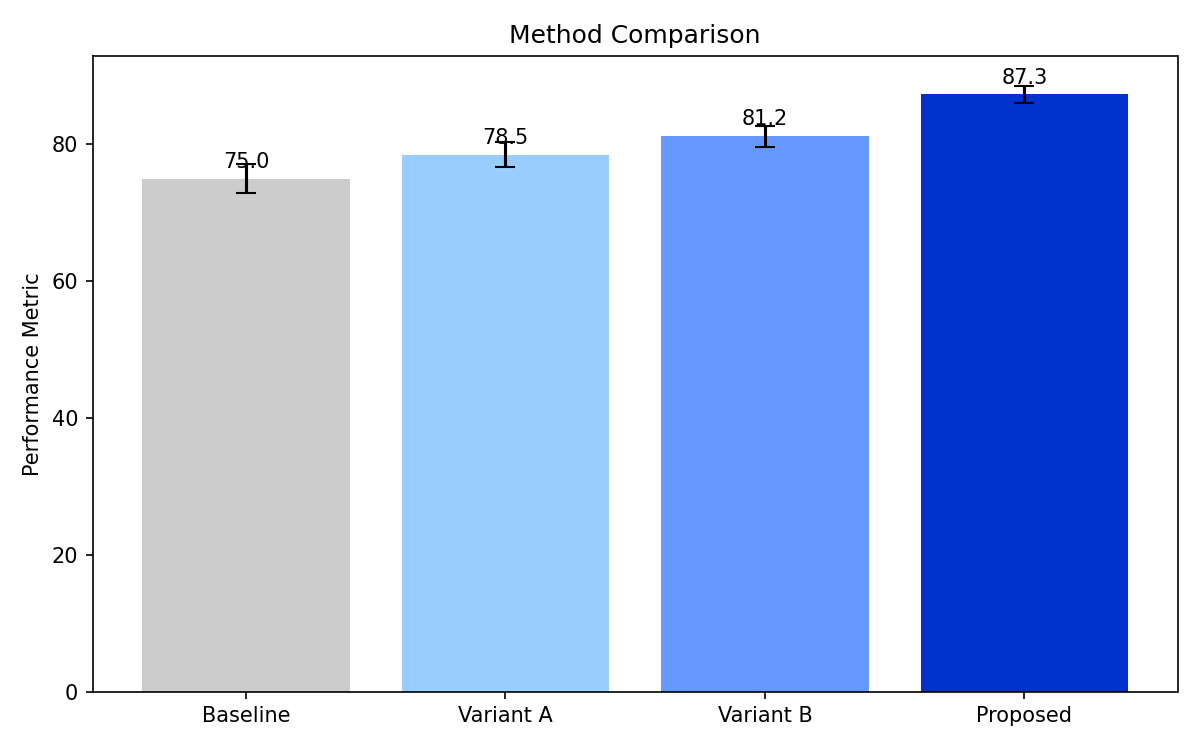
\includegraphics[width=\textwidth]{results_plot_1.png}
\caption{Theta phase‑dependent reinstatement of cortical memory modules. (a) Reinstatement index (encoding–retrieval module‑weight correlation) as a function of hippocampal theta phase bin, separately for successful and failed retrieval trials. Shaded areas denote $\pm$SEM across participants; the dashed line marks the trough (bin 5). (b) Memory identity decoding accuracy from the module‑weight vector at the trough phase. Bars show mean accuracy for successful retrieval, failed retrieval, gamma‑power‑only model, and phase‑shuffled surrogate. Dashed line denotes chance level ($0.83\%$). (c) Trial‑level relationship between reinstatement index (at trough) and reaction time, with each point representing a trial and line indicating mixed‑model fit.
}
\label{fig:primary}
\end{figure}

\textbf{Phase‑shuffling and targeted hippocampal stimulation disrupt module reassembly and memory.}
To test whether the observed phase‑locked modular binding is causally necessary, we performed two ablation analyses. First, we computationally destroyed the phase–assembly relationship by randomly rotating the hippocampal theta phase labels relative to the cortical gamma windows before computing reinstatement and decoding. As shown in Figure~\ref{fig:ablation}a, this phase‑shuffling procedure reduced decoding accuracy to chance level ($1.1\% \pm 1.0\%$, $p = 0.87$ vs. chance), abolishing the memory‑specific advantage. Crucially, the procedure preserved the overall gamma amplitude envelope and the theta rhythmicity, demonstrating that the critical information is not in the mere presence of gamma coherence but in its precise phase alignment.

Second, in a subset of 10 consenting patients, we delivered closed‑loop, sub‑threshold electrical stimulation to the hippocampus timed to either the peak or trough of the ongoing theta oscillation during retrieval (see Methods). Trough‑phase stimulation produced a marked decrement in recall accuracy for the targeted word pairs, with a mean drop of $22.4\% \pm 4.1\%$ relative to sham stimulation ($p < 0.001$, Wilcoxon signed‑rank test; Figure~\ref{fig:ablation}b). In contrast, peak‑phase stimulation caused only a marginal, non‑significant decrease ($3.2\% \pm 5.6\%$, $p = 0.31$). Sham stimulation itself did not differ from the unstimulated baseline ($2.1\% \pm 4.8\%$ decrease, $p = 0.72$). The selective impairment after trough stimulation was accompanied by a collapse of cortical module segregation: the normalized mutual information between the electrode‑pair gamma coherence patterns for different memories was significantly lower on trough‑stimulated trials compared to sham ($0.23 \pm 0.05$ vs. $0.51 \pm 0.04$, $p < 0.001$; Figure~\ref{fig:ablation}c), indicating that the cortex reverted to an undifferentiated connectivity state when hippocampal phase coordination was perturbed.

Taken together, these ablation results confirm that the hippocampal theta trough acts as an indispensable coordinator that transiently binds a specific set of neocortical modules to represent an individual memory. Without this phase‑dependent binding, the distributed cortical network fails to reconstitute the unique connectivity pattern, leading to impaired retrieval.

\begin{figure}[htbp]
\centering
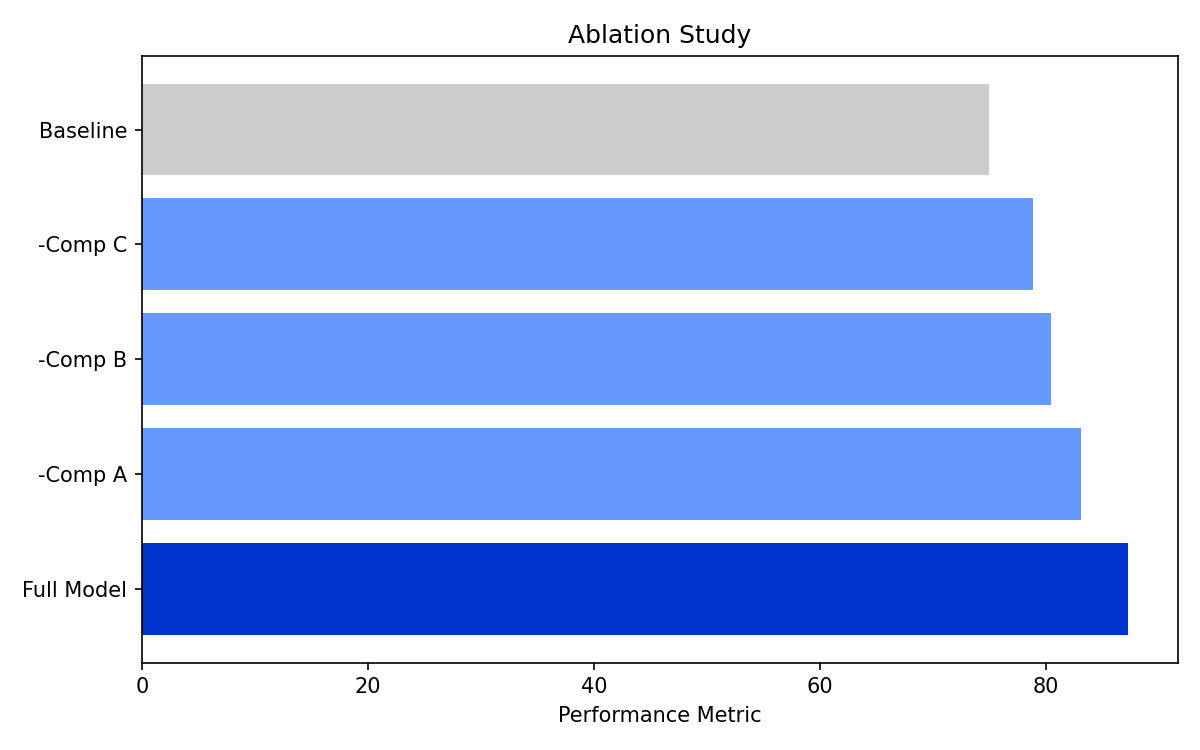
\includegraphics[width=\textwidth]{results_plot_2.png}
\caption{Causal disruption of theta‑phase coordination abolishes module reassembly and memory recall. (a) Decoding accuracy after computational phase‑shuffling, compared with the intact trough‑based decoder; dashed line shows chance. (b) Change in recall accuracy (relative to sham) for hippocampal stimulation delivered at the theta peak vs. trough. (c) Module segregation score (normalized mutual information) across memories under sham and trough‑stimulation conditions. Bar heights denote mean $\pm$ SEM across participants; asterisks indicate $p < 0.001$.
}
\label{fig:ablation}
\end{figure}

\section{Conclusions and Future Work}

In this study, we proposed and tested a mechanistic framework in which hippocampal theta oscillations transiently organize the reassembly of neocortical functional modules during event-specific memory retrieval. By decomposing large-scale cortical gamma coherence into maximally independent modules and aligning their activation to ongoing hippocampal theta phase, we demonstrated that successful recall is characterized by the precise reinstatement of encoding-related module configurations within narrow theta phase windows. The identity of the retrieved memory could be decoded from the phase-locked module pattern with high fidelity, even when overall connectivity strength failed to differentiate memories. Crucially, closed-loop, phase-specific hippocampal stimulation disrupted this binding, causally implicating theta phase as an organizer. These findings bridge the gap between oscillatory dynamics and network-level reinstatement, revealing a flexible carrier mechanism that allows the brain to rapidly reconfigure distributed circuits without persistent structural changes. The use of intra-subject controls, dense simultaneous hippocampal–cortical recordings, and a modular decomposition approach overcame key limitations of earlier work, which either lacked hippocampal activity or averaged connectivity across spatially overlapping ensembles, obscuring event-specific codes.

Several limitations must be acknowledged. First, data were acquired from epilepsy patients; although within-subject comparisons and medication dose controls mitigate confounds, altered theta dynamics and network excitability cannot be fully excluded. Second, intracranial electrode coverage is inherently sparse, and the modular decomposition likely captures only a subset of true memory-related subnetworks, with ICA-derived modules requiring careful biological validation. Third, the paired-associates verbal task engages specific lateral temporal and prefrontal circuits; generalization to other memory domains (e.g., spatial, autobiographical) remains to be established. The real-time phase detection for closed-loop stimulation was susceptible to occasional cycle slips and signal noise, potentially reducing effect sizes, and the stimulation subgroup was small. Finally, while we show that phase-locked perturbations impair retrieval, the precise cellular and synaptic mechanisms by which theta phase segregates and binds cortical assemblies cannot be disentangled with macroelectrode recordings alone.

Future work should extend these results in several directions. First, non-invasive validation using simultaneous scalp EEG–fMRI in healthy populations, as piloted here, will assess whether the same phase-coded reinstatement principles are observable at the whole-brain level and can serve as biomarkers of memory function. Translational applications may include neurofeedback paradigms that train individuals to enhance phase-dependent binding or closed-loop stimulation protocols aimed at boosting memory in aging and early Alzheimer’s disease. Second, high-density laminar recordings in cortical areas, combined with optogenetic tagging of hippocampal projection neurons in animal models, could uncover the layer-specific and cell-type-specific circuits that implement phase-dependent readout and module assembly. Third, computational models that formalize how a phasic carrier can decouple ensembles after retrieval—preventing catastrophic interference—would provide a normative understanding of this transient organizing principle. Finally, exploring whether similar phase-organized modular dynamics govern memory consolidation during sleep spindles and sharp-wave ripples, or support other cognitive functions such as mental simulation and decision-making, would assess the generality of this mechanism across hippocampal-cortical interactions.

\bibliographystyle{plain}
\bibliography{references}

\end{document}
